\subsection{Stakeholder-Analyse}
\subsubsection*{Kommunikation}
Da das Projekt in einer Lernumgebung stattfindet, in der laufende Kommunikation unerlässlich ist, wurden sämtliche Stakeholder ermittelt, welche ein Interesse und einen Einfluss auf das Projekt haben, um abzuwägen, wie extensiv die Kommunikation mit diesen Parteien erfolgen soll.

\begin{itemize}
  \item \textbf{Team} - Das Team, welches die Case-Study durchführt ist für die gesamte Planung, Durch-führung und Auswertung des Projekts verantwortlich. Es hat sehr grosses Interesse am Gelingen dieses Projektes.
  \item \textbf{Kommilitonen} - Die Kommilitonen arbeiten gleichzeitig an Projekten mit denselben Anforderungen. Sie können das Projekt zwar nicht direkt, jedoch indirekt durch den Austausch von Ideen und Problemen beeinflussen.
  \item \textbf{Dozent} - Der Dozent hat durch das Stellen - und allenfalls Verändern - der Aufgabenstellung einen massgeblichen Einfluss auf den Erfolg des Projekts. Dies wird bei dieser Case-Study allerdings dadurch limitiert, dass eine Änderung der Anforderungen nach Projektbeginn ausgeschlossen ist.
  \item \textbf{IBZ} - Die IBZ Schulen AG haben ein relativ geringes Interesse am Projekt an sich, haben aber insofern einen grossen Einfluss darauf, als dass das Projekt abgebrochen werden würde, sollte dies von der Schule verlangt werden. Dieses Szenario ist jedoch sehr unrealistisch.
\end{itemize}

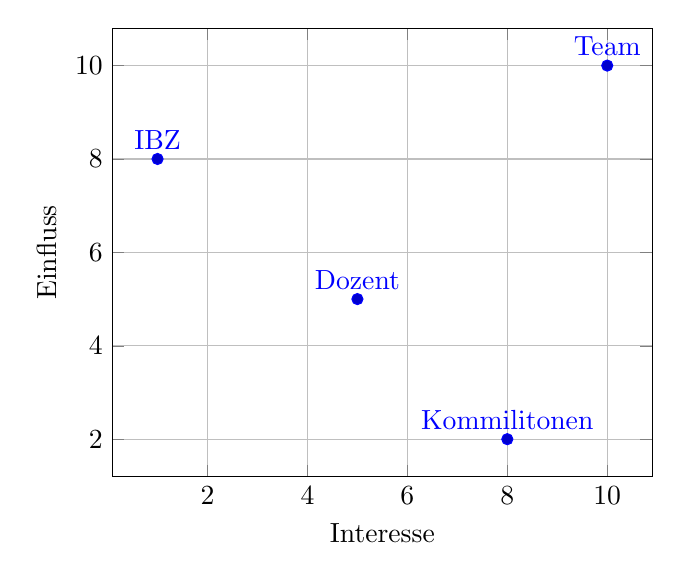
\begin{tikzpicture}
  \begin{axis}[xlabel=Interesse, ylabel=Einfluss, grid=major]
    \addplot+ [nodes near coords,only marks,
    point meta=explicit symbolic]
    table [meta=label] {
    x y label
    10 10 Team
    8 2 Kommilitonen
    5 5 Dozent
    1 8 IBZ
    };
	\end{axis}
\end{tikzpicture}


\subsubsection*{Projektbezogen}
Für die Planung, Lösungs- und Entscheidungsfindung, sowie die nachfolgende Entwicklung werden an dieser Stelle zusätzlich relevanten Stakeholder erfasst.
\begin{itemize}
  \item \textbf{Systemadministrator} - Der Systemadministrator, welcher das System verwaltet, administriert und in unserem Fall (kleines Team) auch allfällige Fehlermeldungen und Anfragen bearbeiten muss.
  \item \textbf{Entwickler} - Der Entwickler, welcher an der [Weiter]entwicklung der Software arbeitet.
  \item \textbf{Reviewer} - Der Entwickler, welchen Code reviewt, bevor er in das Projekt einfliesst.
  \item \textbf{Benutzer} - Der Benutzer, der sein Tagebuch über unsere Plattform erfassen will.
\end{itemize}
